% hydra_circuit_satsuma against satsuma on the SAT Competition 2022
% anniversary track: results of the duo run of 2026-10-04 to 10-11 and a
% stage-by-stage accounting of the PAR-2 difference.
% Build: tectonic doc/hydra_satsuma_2022_anniversary_results.tex
% Numbers and figures: doc/hydra_satsuma_2022_anniversary_figures.py
\documentclass[10pt]{article}
\usepackage[margin=2.4cm]{geometry}
\usepackage{amsmath,amssymb}
\usepackage{booktabs}
\usepackage{array}
\usepackage{enumitem}
\usepackage{microtype}
\usepackage{graphicx}
\usepackage[hidelinks]{hyperref}
\setlist{nosep}
\newcommand{\hcs}{\texttt{hydra\_circuit\_satsuma}}
\newcommand{\sats}{\texttt{satsuma}}
\newcommand{\partwo}{PAR-2}

\title{\bfseries hydra\_circuit\_satsuma on the SAT Competition 2022 Anniversary
  Track:\\ Where the Structural Stages Pay, and What They Cost}
\author{Greg Sidebottom}
\date{October 11, 2026}

\begin{document}
\maketitle

\begin{abstract}
\hcs{} is the SAT Competition 2026 winner, \texttt{satsuma-iter+kissat},
with four certified structural stages in front of it: a Cook prover for
pigeonhole-type shapes, a numeric factoring stage for multiplier circuits,
a GF(2) elimination stage for parity systems, and a circuit stage that
re-encodes hidden multipliers. We ran it beside \sats{} itself on all
5,355 instances of the SAT Competition 2022 anniversary track, the union
of every application, crafted and main track since 2002, with a 5,000 s
limit. \hcs{} solved 4,403 instances to \sats{}'s 4,395, with a \partwo{}
of 1,982.7 against 1,999.3, and eight instances only it solved. Both beat
the 2022 field's virtual best of 4,345 and, after correcting for the Apple
M4 Pro's measured 3.0-fold speed over the competition's StarExec nodes, its
winner by a wide margin. The \partwo{} gap of 16.65 points decomposes exactly: 14.9
points from the eight unique wins, 2.7 from 256 instances the stages
decide in milliseconds where \sats{} searches, and 1.1 points paid as the
stages' prefix on the 5,037 instances they hand on. Only 8 of the 264
instances the stages decide became unique wins because \sats{}'s symmetry
breaking refutes 207 of them by itself; the eight are the parity formulas
wrapped in cardinality constraints and the two largest mutilated
chessboards, where that breaking finds nothing. Nearly half of the cost
was a bug, fixed after the run.
\end{abstract}

\section{Introduction}

The companion document \texttt{hydra\_satsuma\_solver} describes the
solver and its results on the 2026 main track, where \hcs{} solves four
more instances than \sats{} out of 391. A 391-instance set with four
unique wins says little about where the stages pay in general, so we ran
the same two solvers over the 2022 anniversary track~\cite{sc22}, the
largest benchmark set the competition has published: 5,355 instances from
133 families, covering twenty years of application, crafted and main
tracks. The run took seven days on ten cores. This document reports the
result and answers the question the run was designed for: for each stage,
on how many instances did it help, by how much, and what did it cost on
the instances where it did not.

\section{The two solvers}

\sats{} is \texttt{satsuma-iter+kissat} as submitted to the 2026
competition~\cite{sbr}: satsuma's symmetry preprocessing in its iterative
mode, which detects symmetries with dejavu and adds units, binary and
lex-leader clauses with a binary substitution-redundancy proof, followed
by kissat, whose refutation is appended to the same proof. We run the
official image unchanged. Our \texttt{sat} binary parses the formula,
writes it to the container, runs the official script, and projects a model
back to the original variables.

\hcs{} runs four stages on the parsed formula before handing it to that
same engine, byte for byte:
\begin{enumerate}
\item the \emph{Cook prover}: recognisers for pigeonhole, embedded
  pigeonhole, round-robin, clique-colouring and mutilated chessboard
  shapes, each refuted by a short cutting-planes argument written as a
  VeriPB proof~\cite{cook76,haken85};
\item the \emph{factoring stage}: multiplier recognition and numeric
  factoring of the output constant, which decides a factoring instance
  with the model as certificate;
\item the \emph{XOR stage}: recovery of complete parity encodings and
  Gaussian elimination over GF(2); an inconsistent system is refuted with
  a Gocht--Nordstr\"om parity proof~\cite{gn21}, a consistent pure-XOR
  formula gets its model from back-substitution~\cite{tseitin68,urquhart87,soos09};
\item the \emph{circuit stage}: trial factoring of the gate structure to
  find hidden multipliers, and a certified re-encoding when enough are
  found; it fires on none of the 5,355 instances, so here it is pure cost.
\end{enumerate}
Each stage either decides the instance with a certificate or hands the
unchanged formula to the next; the engine sees the original formula. In
this run certificate checking was off: the stage proofs were written, not
checked. In the October 2026 main-track run with checking on, all 27 Cook
and 11 XOR certificates verified under VeriPB, and \sats{}'s own
certificates are checked by \texttt{dsr-trim} there.

\section{The benchmark and the protocol}

\paragraph{Instances.} All 5,355 instances of the anniversary track, in
GBD's order (sorted by hash, which mixes the families), with GBD's recorded
status for 4,715 of them. The two solvers' answers agree with every
recorded status.

\paragraph{Machine and limits.} An Apple M4 Pro (10 performance and 4
efficiency cores, 64\,GB), ten jobs at a time so no job lands on an
efficiency core. The engine runs in Docker Desktop with a 32\,GB VM; a
memory-aware scheduler admits instances by estimated footprint against a
26\,GB VM budget and a 20\,GB host budget. 5,000 s of wall-clock per
instance and solver, \partwo{} scoring (an unsolved instance counts
10,000 s).

\paragraph{Pairing.} \texttt{tools/gbd/duo.py} runs both solvers through
the set in the same order and starts the two jobs of an instance together,
so they meet the same machine load. The 54 instances that started before
the switch to pairing, three hours in, and that no stage decided were run
in full by both. From then on \hcs{} ran only its stages: when they hand the
formula on, its result is \sats{}'s on the identical formula, and its time
is its own prefix plus \sats{}'s engine time. This is exact rather than an
approximation: the engine's input is byte-identical, and satsuma and
kissat are deterministic on identical input, which we checked on the full
pairs. It halved the compute and, more importantly for this document,
gives the prefix of every hand-off as a measured number.

\paragraph{Speed against 2022.} The anniversary track ran on StarExec's
Intel Xeon E5-2609 nodes (2.4\,GHz, 2012) and reports CPU seconds. To
compare counts under the same 5,000 s limit we timed the 2022 track's
most-solved solver, \texttt{kissat-sc2022-bulky}, built from its
competition tag, on twenty anniversary instances spread over families and
solve times, in the same Docker VM at the same ten-job load. Its search
does not depend on time, so the ratio of its times is the hardware's: the
median was 2.99, quartiles 2.79 to 3.12, range 1.82 to 3.83, with every
verdict as recorded. We use 3.

\paragraph{Timeline.} The run started 2026-10-04 14:23 on eight cores,
switched to the paired-reuse protocol at 17:18, to ten cores at 22:30, and
finished 2026-10-11 15:08, after seven days and 39 minutes of activity at a
mean pace of about 32 instances per hour. Two events cost capacity and
nothing else: half an hour at nine cores for the speed calibration, and 53 minutes on
10-06 during which a scheduler bug held the queue behind one job and three
jobs ran instead of ten. A cheaper implementation of the circuit stage's
check, with identical results, was installed after 164 instances.

\section{Results}

\begin{table}[h]
\centering
\begin{tabular}{lrrrrr}
\toprule
 & solved & SAT & UNSAT & unsolved & \partwo{} \\
\midrule
\sats{} & 4,395 & 1,990 & 2,405 & 960 & 1,999.3 \\
\hcs{} & \textbf{4,403} & 1,991 & 2,412 & 952 & \textbf{1,982.7} \\
\midrule
2022 virtual best (28 solvers) & 4,345 & 2,140 & 2,205 & 1,010 & 2,108.5 \\
2022 winner, Kissat\_MAB\_ESA & 4,028 & & & & 2,806.4 \\
2022 most solved, kissat-sc2022-bulky & 4,037 & & & & 2,811.0 \\
\bottomrule
\end{tabular}
\caption{All 5,355 instances. The 2022 rows are the competition's own
times on StarExec, so their counts compare with ours only after the
speed correction of Section~\ref{sec:field}. The virtual best takes the
fastest of the 28 sequential entrants on each instance.}
\label{tab:score}
\end{table}

Table~\ref{tab:score} gives the score. \hcs{} solves eight more instances
than \sats{} and loses none: every instance \sats{} solves, \hcs{} solves,
because the engine is the same and the stages only ever decide an instance
or step aside. Figure~\ref{fig:cactus} is the cactus plot. The eight
instances only \hcs{} solved are in Table~\ref{tab:unique}; all eight are
decided in milliseconds by a stage, and \sats{} ran the full 5,000 s on
each. None of the 28 solvers of 2022 solved seven of them; mchess\_20 was
solved by seven.

\begin{table}[h]
\centering
\begin{tabular}{llllr}
\toprule
instance & family & stage & \hcs{} & 2022 \\
\midrule
pmg-14 & long-learned-clauses & XOR, parity proof & 6.0 ms & 0/28 \\
eulcbip-8 & long-learned-clauses & XOR, parity proof & 5.2 ms & 0/28 \\
mchess\_20 & mutilated-chessboard & Cook, VeriPB & 1.9 ms & 7/28 \\
pmg-13 & long-learned-clauses & XOR, parity proof & 6.9 ms & 0/28 \\
mod2-rand3bip-sat-300-3 & tseitin-formulas & XOR, model & 0.6 ms & 0/28 \\
eulcbip-9 & long-learned-clauses & XOR, parity proof & 6.7 ms & 0/28 \\
eulcbip-7 & long-learned-clauses & XOR, parity proof & 4.2 ms & 0/28 \\
mchess\_19 & mutilated-chessboard & Cook, VeriPB & 1.6 ms & 0/28 \\
\bottomrule
\end{tabular}
\caption{The eight instances \hcs{} solved and \sats{} did not, in run
order. The last column is how many of the 28 solvers of 2022 solved the
instance.}
\label{tab:unique}
\end{table}

\begin{figure}[h]
\centering
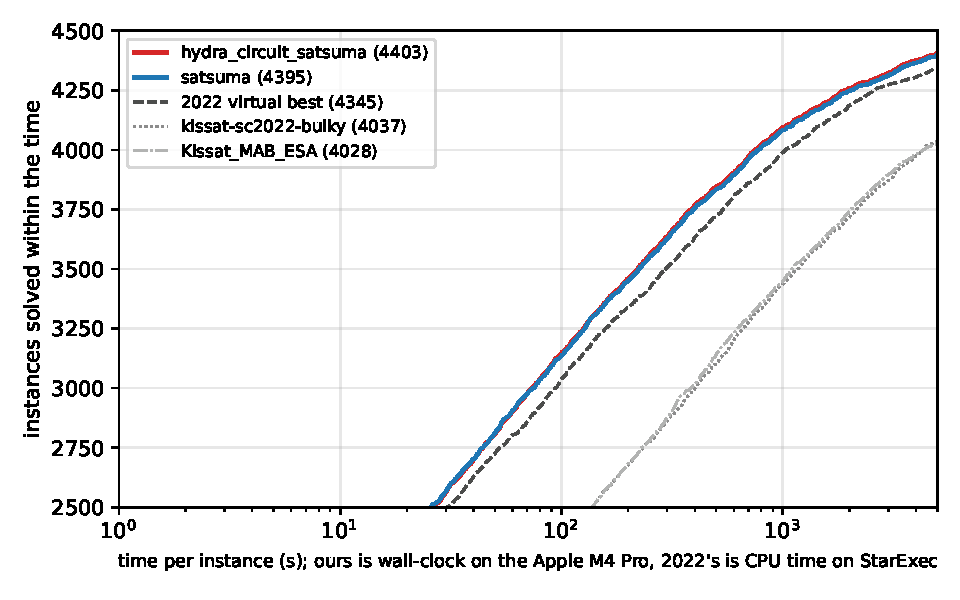
\includegraphics[width=0.8\linewidth]{hydra_satsuma_2022_anniversary_cactus.pdf}
\caption{Instances solved within a per-instance time. Ours are wall-clock
times on the Apple M4 Pro; the 2022 curves are CPU seconds on StarExec's
Xeon E5-2609 nodes, about three times slower per job, so they sit to the
right of where they would on the M4 Pro.}
\label{fig:cactus}
\end{figure}

Beyond the uniques, the two arms differ on the 264 instances a stage
decides and on nothing else. On the other 256 of those, \sats{} also
solves the instance and \hcs{} is faster every time: the stages' median
time on the 264 is 4.6 ms and their maximum 229 ms, against \sats{}'s
median of 0.34 s on the XOR-decided instances, 0.36 s on the Cook-decided
ones and 21 s on the factoring ones. The large differences are the
instances \sats{} solves slowly: mchess\_17 in 4,179 s, the satisfiable
random parity system mod2-rand3bip-sat-290-2 in 4,057 s, pmg-12 in
3,063 s, mod2-rand3bip-sat-270-3 in 585 s, the factoring instance
10142772393204023nc in 489 s, mchess\_18 in 341 s. Everywhere else
\hcs{} is \sats{} plus a prefix. The geometric mean of the time ratio
\hcs{}/\sats{} over the 2,543 instances both solved in at least 5 s is
1.042: the prefix, which is at most a few seconds except where a stage
misbehaves (Section~\ref{sec:cost}).

\section{Where the \partwo{} difference comes from}
\label{sec:account}

The \partwo{} gap is $1{,}999.3 - 1{,}982.7 = 16.65$ points, which is
$89{,}150$ s of the summed score over 5,355 instances. Since the two arms
share the engine, every instance falls into one of four classes, and the
sum of the per-instance differences over the classes is the gap exactly.
Table~\ref{tab:account} and Figure~\ref{fig:contrib} give the
decomposition, with each class split by stage.

\begin{table}[h]
\centering
\begin{tabular}{llrrr}
\toprule
class & stage & instances & seconds & \partwo{} points \\
\midrule
unique wins & XOR & 6 & $+60{,}000$ & $+11.20$ \\
 & Cook & 2 & $+20{,}000$ & $+3.73$ \\
speed wins (both solve, the stage decides) & XOR & 161 & $+8{,}715$ & $+1.63$ \\
 & Cook & 82 & $+4{,}909$ & $+0.92$ \\
 & factoring & 13 & $+835$ & $+0.16$ \\
full-run pairs (before pairing) & & 54 & $-64$ & $-0.01$ \\
prefix on hand-offs & factoring trial & 5,037 & $-73$ & $-0.01$ \\
 & XOR stage & 5,037 & $-2{,}827$ & $-0.53$ \\
 & circuit trial & 4,866 & $-2{,}997$ & $-0.56$ \\
 & other & 5,037 & $-183$ & $-0.03$ \\
\midrule
total & & 5,355 & $+89{,}150$ & $+16.65$ \\
\bottomrule
\end{tabular}
\caption{The \partwo{} gap decomposed. Seconds are the summed difference
$\text{score}(\sats) - \text{score}(\hcs)$ over the instances of the row;
points divide by 5,355. A unique win is worth 10,000 s minus the stage's
milliseconds. The circuit trial runs on the 4,866 hand-offs with at most
10 million clauses; the 171 larger ones skip it. ``Other'' is the
hand-off time the per-stage lines do not account for: the Cook recognisers
on a miss, XOR recovery when it finds nothing, and clause copies.}
\label{tab:account}
\end{table}

\begin{figure}[h]
\centering
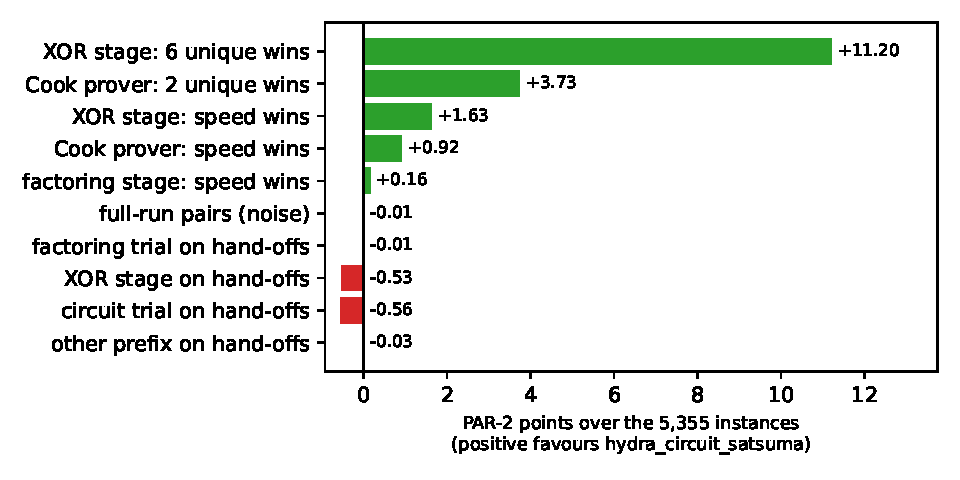
\includegraphics[width=0.78\linewidth]{hydra_satsuma_2022_anniversary_contributions.pdf}
\caption{The rows of Table~\ref{tab:account}.}
\label{fig:contrib}
\end{figure}

Three things stand out.

\paragraph{Unique wins dominate.} Each is worth $10{,}000/5{,}355 = 1.87$
points, and the eight are 14.9 of the 16.65. A stage that solves one
instance \sats{} cannot is worth more than the stages' total cost over the
whole set, and worth more than all 256 speed wins together. The speed wins
are the stages' everyday business, 256 instances decided in milliseconds,
but \sats{} already solves most of them in under a second, so they add
2.7 points.

\paragraph{The cost is small, and most of it was avoidable.} The 5,037
hand-offs paid 6,080 s of prefix in total, a mean of 1.21 s and 1.14
points. 1,124 hand-offs paid more than a second and 73 more than ten.
Section~\ref{sec:cost} traces the cost to two sources, a bug now fixed and
the circuit trial.

\paragraph{The full-run pairs are noise.} On the 54 instances both arms
ran in full, \hcs{} pays its prefix and then runs the same deterministic
search; the net is $-64$ s, 43 of the 54 slightly in \sats{}'s favour.
Their spread, a few seconds per instance, is the measurement noise of two
jobs sharing the M4 Pro with eight others.

\section{Why only eight of 264}
\label{sec:why}

The stages decide 264 instances: 167 by the XOR stage (155 refutations,
12 satisfiable pure-XOR systems), 84 by the Cook prover and 13 by
factoring. Of these, 129 were solved by none of the 28 solvers of 2022,
yet only 8 became unique wins. The reason is \sats{}'s symmetry breaking,
and we can measure it: we ran satsuma's symmetry step alone, with the
competition's flags and without kissat, on all 264
(\texttt{tools/gbd/sym\_probe.py}).

\begin{table}[h]
\centering
\small
\begin{tabular}{lrrrrl}
\toprule
symmetry step alone & $n$ & solved & median & max & failed \\
\midrule
derives the empty clause & 207 & 207 & 0.33 s & 13.8 s & none \\
adds clauses, no refutation & 30 & 25 & 11.9 s & 4,180 s & eulcbip-7, -8, -9; mchess\_19, \_20 \\
finds no symmetry & 27 & 24 & 24.1 s & 4,057 s & pmg-13, -14; mod2-rand3bip-sat-300-3 \\
\bottomrule
\end{tabular}
\caption{The 264 stage-decided instances by what satsuma's symmetry step
does on its own, with \sats{}'s result in the run. The probe was made at
instance 660 of the run and predicted the remaining unique wins: the six
it rated strong all landed, one of its two likely candidates did
(pmg-12 was solved in 3,063 s), and none of its low ones.}
\label{tab:probe}
\end{table}

Table~\ref{tab:probe} gives the result. On 207 of the 264 the symmetry step
alone derives the empty clause, and \sats{} solved every one, in a median
of 0.33 s. These are the Tseitin, Urquhart and xor-chain formulas written
as plain XOR clauses, and the pigeonhole and clique-colouring families: in
a plain Tseitin encoding every variable sits in exactly two parity
constraints, so flipping the edges around any cycle of the graph is a
symmetry, and breaking those symmetries is a refutation. Our XOR stage
refutes the same instances in milliseconds, but \sats{} refutes them in a
second, so they are speed wins.

The unique wins are where that mechanism breaks:
\begin{itemize}
\item \textbf{pmg} and \textbf{eulcbip} are Tseitin formulas inside
  cardinality constraints: exactly one of three edges at each vertex in
  pmg, exactly two of four in eulcbip, with one twisted pair making the
  total parity odd. Each vertex's clauses contain a complete XOR encoding,
  which the XOR stage reads, plus extra clauses that destroy the cycle
  flips. satsuma finds no symmetry on pmg-13 and pmg-14 and fixes one
  variable on the eulcbip instances, so kissat meets a parity formula at
  full strength, which resolution cannot refute in polynomial
  size~\cite{urquhart87}. pmg-12, the smallest, was the exception: 63
  binary symmetry clauses were enough for kissat to finish, in 3,063 s.
\item \textbf{mchess\_19} and \textbf{mchess\_20} are the largest
  mutilated chessboards; satsuma fixes two variables on each. \sats{}
  solved mchess\_15 to 18 in 84 to 4,179 s, in the 2022 field's difficulty
  order, and ran out of time on 19 and 20. The Cook prover counts squares
  of two colours~\cite{cook76}.
\item \textbf{mod2-rand3bip-sat-300-3} is a satisfiable random parity
  system with every variable in three equations, so no flips exist and the
  outcome is search luck: \sats{} solved the ten smaller members, in 3.9 s
  to 4,057 s, eight of them slower than the 2022 field's best time, and
  timed out on this one, which two of 28 solvers solved in 2022.
\end{itemize}

The lesson for future stages is a measurement, not a family list: a
stage is worth building where the engine's own preprocessing has no
purchase, and satsuma's symmetry step alone, run on candidate instances,
tells which those are before any engine time is spent.

\section{The cost, and where it went}
\label{sec:cost}

The prefix of a hand-off is parse-free: the clock starts after parsing,
which both arms do identically. It is the four stages' work on a formula
they then hand on.

\paragraph{The XOR stage, 2,827 s.} On a mixed formula whose parity
system is consistent, the stage propagated the elimination's forced units
through the whole formula with a fixpoint loop over all clauses, to build
a simplified residual, and then discarded the residual because in
certified mode the engine must refute the original formula. On the
bitvector family the ``system'' is a single recovered unit clause and the
loop cascaded it through two to three million clauses: 201 s on
bvult\_16967, 199 s on bvslt\_19860, 110 to 136 s on the bvadd instances,
40 to 67 s on shift1add. That discarded propagation is 2,637 s of the
stage's 2,827 s and 0.49 of the gap's points; kissat does the same
propagation in under a second. It is fixed: the stage now returns right
after the elimination when the residual cannot be used
(\texttt{solve\_xor\_system(.., simplify\_mixed=false)}), which brings
bvult\_16967's hand-off from 202.8 s to 2.6 s with identical verdicts, and
would have made the gap 17.1 points. The bitvector family is the only one
where \hcs{} lost ground, $-1{,}608$ s over 216 instances.

\paragraph{The circuit trial, 2,997 s.} The circuit stage's trial
factoring runs on every hand-off with at most ten million clauses and
found a multiplier worth rewriting on none; the anniversary set predates
the GenMul encodings it was built for, which entered the competitions in
2025. Its cost is spread thin, 0.6 s per instance, with the largest on the
core-based-generator and planning instances with millions of gates
(ncc\_none\_7047, 42 s; two more ncc instances, 24 s each; atco\_enc3, 22 s).
It is the one remaining cost worth gating, by the gate count or by
stopping the trial early when the first products do not appear; at
0.56 points it is a third of a unique win.

\paragraph{Everything else, 256 s.} The factoring stage's trial (73 s over
5,037 instances), the Cook recognisers and XOR recovery on misses, and the
clause copies between stages cost 0.05 points together. The Cook prover,
whose two unique wins and 82 speed wins are worth 4.65 points, costs
nothing measurable.

\section{Against the 2022 field}
\label{sec:field}

Both arms solved more instances than the 2022 virtual best, 4,403 and
4,395 against 4,345, on an M4 Pro three times faster per job than the
competition's Xeon E5-2609 nodes. Scaling our
times by a factor $k$ and recounting under the 5,000 s limit says how much
of that is the hardware. \sats{} keeps more solved instances than the 2022
winner Kissat\_MAB\_ESA while $k \le 5.85$ and a lower \partwo{} while
$k \le 5.46$; \hcs{} while $k \le 6.13$ and $5.64$. At the measured
$k = 3$ the counts are 4,201 and 4,212 with \partwo{} 2,461 and 2,442,
against the winner's 4,028 and 2,806. Even the largest ratio measured,
3.83, leaves both ahead. The virtual best is another matter: it is the
best of 28 solvers on each instance, and both arms fall behind its count
once $k$ exceeds 1.43 (\sats{}) or 1.49 (\hcs{}). \hcs{} solved 248
instances that no 2022 solver solved, \sats{} 242, and each missed about
190 that some 2022 solver solved.

\section{What the run says about the next stages}

Five candidate stages were listed before the run with the anniversary
instances they target, so that \sats{}'s results would rank them
(\texttt{doc/ideas\_watchlist.md}, \texttt{tools/gbd/watchlists.py}). A
stage pays only where \sats{} fails, at 1.87 points per instance here.

\begin{itemize}
\item \emph{Near-complete parity systems}, 21 instances: Tseitin, Urquhart
  and xor-chain formulas with one clause removed, so one parity is
  incomplete and the XOR stage hands on. \sats{} failed all 21, as did all
  of 2022. Gaussian elimination over the complete parities with the
  incomplete one as clauses, or a case split on its missing row, is the
  obvious stage; the symmetry probe explains why satsuma fails them, the
  missing clause kills the cycle flips.
\item \emph{Equivalence chains}, 10 instances (equilarge): \sats{} failed
  all 10.
\item \emph{Algebraic multiplier miters}, 23 instances with explicit
  partial products: \sats{} failed 16. The known method is algebraic
  (AMulet-style polynomial reduction with PAC certificates), a larger
  build.
\item \emph{Cook recognisers for more encodings}, 113 instances: \sats{}
  failed 7, five relativised pigeonhole and two clique-colouring
  variants. Its symmetry breaking took the other 106, so this idea shrank
  from 56 unsolved-in-2022 targets to 7.
\item \emph{A bounded local-search stage}, 35 satisfiable instances a
  walk-heavy 2022 solver took quickly: \sats{} failed 27, but a walk would
  rescue only some, at a cost on every instance.
\end{itemize}

The first two are the same mechanism as this run's unique wins, parity
reasoning where symmetry breaking has nothing to break, and together they
are 31 instances no entrant of 2022 or \sats{} solves.

On the newer competition sets the density is higher: 4 unique wins in 391
instances on the 2026 main track, and a scan of the 2025 main track with
the same probe predicts 4 to 5 of 400, three of them Tseitin grids of
124,500 to 319,200 variables on which satsuma's symmetry step finds a few
dozen generators and the XOR stage finishes in 64 to 556 s
(\texttt{doc/data/main\_2025\_stage\_scan.md}).

\section{Conclusion}

On the broadest set the competition has, the structural stages cost
1.1 \partwo{} points and gained 17.6, almost all of it from eight
instances no engine solves and the stages decide in milliseconds. The
cost was 6\% of the gain before the fix and will be about 4\% after it.
The stages did not lose a single instance, and their
certificates are the same VeriPB and parity proofs that verified in the
2026 run. The limiting factor is the number of instances where structure
is the only way in: \sats{}'s symmetry breaking already takes the easy
parity and pigeonhole formulas, which is exactly why the two families
behind this run's eight wins, parity under cardinality and the largest
chessboards, and the 31 near-complete parity and equivalence-chain
instances still open, are the right next targets.

\paragraph{Artifacts.} Run directory
\path{sat_benchmarks/runs/anni_2022_duo} (results, per-job logs, stage
scan, symmetry probe); reports in \path{doc/competition/}
(\path{duo_anni_2022_5000_satsuma_vs_hydra_circuit_satsuma.md} and the two
per-solver reports); the numbers and figures of this document from
\path{doc/hydra_satsuma_2022_anniversary_figures.py}; the speed
calibration in \path{doc/data/speed_calibration_sc2022.md}.

\begin{thebibliography}{99}
\setlength{\itemsep}{2pt}

\bibitem{sc22} T.~Balyo, M.~J.~H. Heule, M.~Iser, M.~J\"arvisalo, and
  M.~Suda (eds.).
\newblock Proceedings of SAT Competition 2022: Solver and Benchmark
  Descriptions.
\newblock University of Helsinki, 2022. Results and detailed per-instance
  data: \url{https://satcompetition.github.io/2022/}.

\bibitem{sbr} M.~Anders, C.~Codel, and M.~J.~H. Heule.
\newblock Simplify, order, break, repeat.
\newblock \emph{SAT 2026}, LIPIcs vol.~377, article~4. satsuma:
  \url{https://github.com/markusa4/satsuma}; the SAT Competition 2026
  winner \texttt{satsuma-iter+kissat}:
  \url{https://satcompetition.github.io/2026/downloads/solvers/anders.tar.xz}.

\bibitem{cook76} S.~A. Cook.
\newblock A short proof of the pigeon hole principle using extended
  resolution.
\newblock \emph{SIGACT News}, 8(4):28--32, 1976.

\bibitem{haken85} A.~Haken.
\newblock The intractability of resolution.
\newblock \emph{Theoretical Computer Science}, 39:297--308, 1985.

\bibitem{gn21} S.~Gocht and J.~Nordstr\"om.
\newblock Certifying parity reasoning efficiently using pseudo-Boolean
  proofs.
\newblock \emph{AAAI}, 2021.

\bibitem{tseitin68} G.~S. Tseitin.
\newblock On the complexity of derivation in propositional calculus.
\newblock \emph{Studies in Constructive Mathematics and Mathematical
  Logic, Part II}, pp.~115--125, 1968.

\bibitem{urquhart87} A.~Urquhart.
\newblock Hard examples for resolution.
\newblock \emph{Journal of the ACM}, 34(1):209--219, 1987.

\bibitem{soos09} M.~Soos, K.~Nohl, and C.~Castelluccia.
\newblock Extending SAT solvers to cryptographic problems.
\newblock \emph{SAT}, LNCS 5584, pp.~244--257, 2009.

\end{thebibliography}

\end{document}
